\documentclass[11pt, a4paper]{article}

\usepackage[utf8]{inputenc}
\usepackage[T1]{fontenc}
\usepackage{geometry}
\usepackage{graphicx}
\usepackage{xcolor}
\usepackage{tcolorbox}
\usepackage{hyperref}
\usepackage[backend=biber, style=numeric]{biblatex}
\addbibresource{references.bib}

% Define git-like colors
\definecolor{gitdark}{HTML}{0F0F0F}
\definecolor{gitlight}{HTML}{E1E1E1}
\definecolor{gitred}{HTML}{F92672}
\definecolor{gitgreen}{HTML}{A6E22E}
\definecolor{gitblue}{HTML}{66D9EF}
\definecolor{gitorange}{HTML}{FD971F}

% Set page geometry
\geometry{left=25mm,right=25mm,top=20mm,bottom=20mm}

% Customize hyperlinks
\hypersetup{
    colorlinks=true,
    linkcolor=gitblue,
    filecolor=gitmagenta,
    urlcolor=gitblue,
}

% Custom tcolorbox environments
\newtcolorbox{gitbox}[1][]{
    colback=gitdark,
    colframe=gitgreen,
    coltext=gitlight,
    boxrule=0.5pt,
    #1
}

% Customize section color
\usepackage{sectsty}
\sectionfont{\color{gitgreen}}

% Set overall page color
\pagecolor{gitdark}
\color{gitlight}

% Use XeTeX or LuaTeX and set a custom font (Inconsolata in this example)
%\usepackage{fontspec}
%\setmonofont{Inconsolata}

\begin{document}

    \title{\color{gitred}Proposal for Re-Use and Re-Design Flawed Reward System}
    \author{\color{gitgreen}Your Name}
    \date{\color{gitorange}\today}
    \maketitle

    \tableofcontents
    \newpage
    \begin{figure}
        \centering
        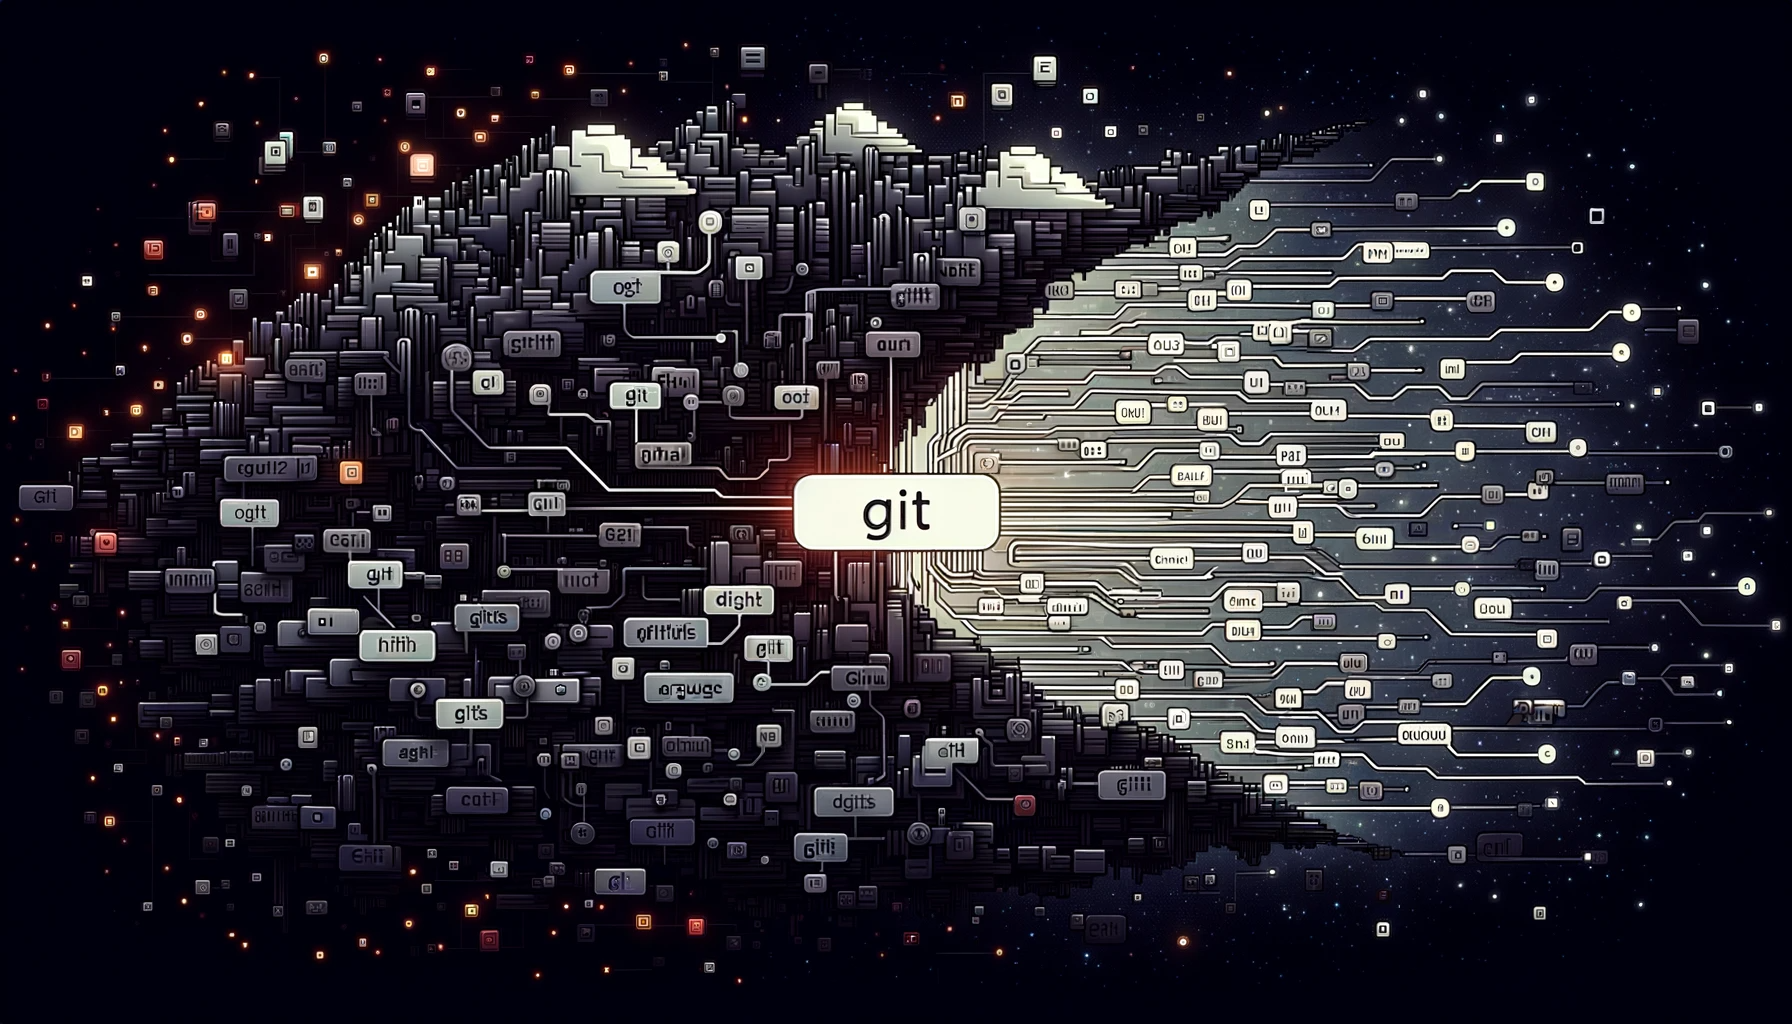
\includegraphics[width=\textwidth]{/home/kilian/Dokumente/Git/graph_to_agent/READ_ME/assets/the_git}
        \caption[Beacon of Git]{Git-approach to bring light into our scrollable, short-lived world}
        \label{fig:}
    \end{figure}



    \begin{gitbox}
        \section*{Abstract}
        Let's enumerate in one section what this is all about (yes, we do repeat Personal Knowledge Library (PKL) definition on purpose):

        \begin{itemize}
            \item \textbf{Overarching Goal}: A social-network consisting of Knowledge Graphs in the form of Personal Knowledge Libraries (PKL)
            \item \textbf{Public Section of Personal Knowledge Library (PKL)} as a way to build up knowledge adhering to "standing on the shoulders of giants"
            \item \textbf{Git-Approach to Personal Knowledge Library (PKL)} adheres to "cross-validation" principles, by forking out, reassessing and making a pull-request/ merge back in the original Personal Knowledge Library (PKL)
            \item By visualizing the intellectual trajectories of thought and discovery in the Public Section of the Personal Knowledge Library (PKL), we enable some kind of "reproducibility"
            \item Use The Wire-Box [link] or Augmented Argumentation via Agent Interactions to encapsulate expert knowledge and an infinite universe of further options
            \item Plot and re-use a flawed reward system
        \end{itemize}
    \end{gitbox}

    \begin{gitbox}[colframe=gitred]
        \section*{The Problem}
        Today's "infinite scroll"/"slot-machine" presents content—whether posts, images, or videos—in a seemingly endless, disconnected stream. This disconnect impedes users from delving into interconnected topics, depriving them of a cohesive understanding. Furthermore, most of these platforms and even more scientific ones e.g., nature journal, are triggered by the rewards of quick wins \& news coverage. Such superficial and short-lived scrolling news contrasts sharply with Knowledge Graphs, where interconnected pathways usher users to deeper insights and to track the history \& performance of news-commits.
    \end{gitbox}


    \begin{gitbox}
        \section*{Solution Pillars}
        \begin{itemize}
            \item \textbf{Personal Knowledge Libraries (PKL)}: Example: Imagine Instagram's chronological photo feed, but instead of photos, you have nodes representing key thoughts, ideas, or memories. Or consider LinkedIn, where connections don't just represent professional relationships, but conceptual links between ideas. In essence, PKL isn’t just another social media platform—it's a fusion that amalgamates the essence of Instagram's visual storytelling, Twitter's/ X's bite-sized thoughts, LinkedIn's professional sharing, and even Tinder's interactive engagement, all aimed at charting the growth of a person's intellectual journey.
        \end{itemize}
    \end{gitbox}

    \begin{gitbox}
        \section*{Immediate Goals}
        One immediate goal is to design a platform for a knowledge graph generation with a simple, maintainable pipeline for content (blobs) to graph integration. This includes modules such as 'Time-Stamped Content Evolution Graphs' and 'Augmented Argumentation via Agent Interactions,' with the option to segregate between private and public repositories, allowing users to control what they share.
    \end{gitbox}

    \begin{gitbox}
        \section*{Future Vision}
        Pair PKL with virtual reality to visualize a personal 3D knowledge universe, creating an immersive narrative of evolving thoughts. Imagine navigating a cerebral museum, where every node and connection brings to life the intellectual universe. This could aid others facing similar problems and life stages.
    \end{gitbox}
    \begin{figure}
        \centering
        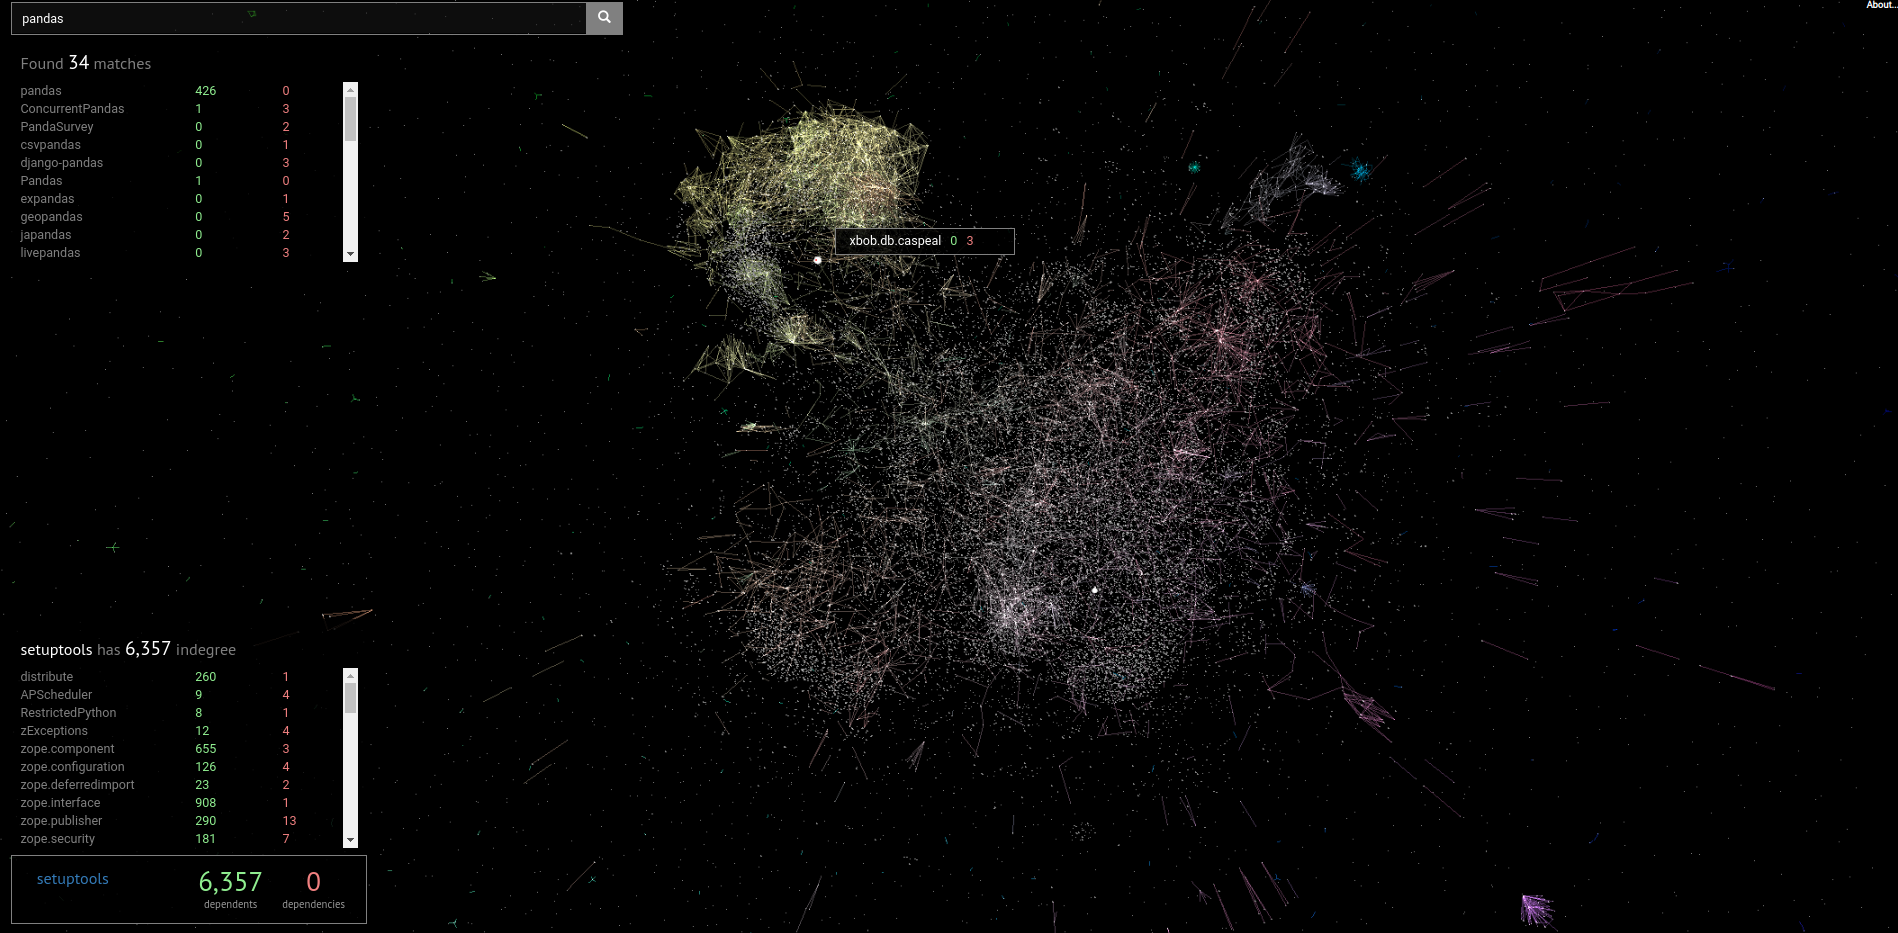
\includegraphics[width=\textwidth]{/home/kilian/Dokumente/Git/graph_to_agent/READ_ME/assets/enter_py_universe}
        \caption{View on "Code Galaxies Visualization" by Andrei Kashcha}
        \label{fig:}
    \end{figure}

    \begin{gitbox}
        \section*{Time-Stamped Content Evolution Graphs}
        Consider how narratives such as 'A Dangerous Game' and 'Arrival' challenge conventional understandings of time. These works suggest a more fluid conception of time, which invites a re-evaluation of our experiences. Politicians’ shifting speeches and the prevalence of 'Fake News' complicate discerning fact from fiction. Our git-versioned content graph system records 'commits' of content from specific sources at specified times, allowing users to trace narrative evolution and recognize patterns.

        Current Status: MVP in Development.
    \end{gitbox}

    \begin{gitbox}
        \section*{The Wire-Box or Augmented Argumentation via Agent Interactions}
        Envision a box of wires, akin to neural connections in our brain. These represent the edges, links, and pathways of thoughts that users can customize. Users can segment their thought processes, encapsulate them within agents, and interlink them. For example, tracking a politician's statements on climate change could involve agents for environmental data, socio-economic implications, and global political reactions. These agents are interconnected facets of understanding, mimicking internal dialogues for complex topics.


        Current Status: MVP Available [here](link to MVP).
    \end{gitbox}

%    \begin{figure}[ht]
%        \centering
%        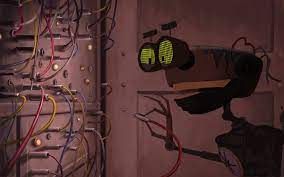
\includegraphics[width=\textwidth]{/home/kilian/Dokumente/Git/graph_to_agent/READ_ME/assets/wire_it_treasure_planet}
%        \caption{Wire-it Ben!}
%    \end{figure}

%    \begin{figure}[ht]
%        \centering
%        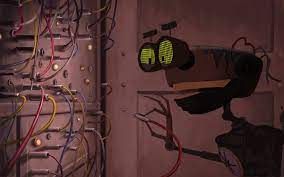
\includegraphics[width=200,height=100]{/home/kilian/Dokumente/Git/graph_to_agent/READ_ME/assets/wire_it_treasure_planet}
%        \caption{}
%    \end{figure}

    \begin{gitbox}
        \section*{Why the Wire-Box}
        The Wire-Box was designed with the vision of enabling non-technical users to utilize graph-based agent behavior. It's not just about using expert knowledge but allowing experts in various fields to apply their expertise in a meaningful way. The idea is to enable experts to unlock knowledge encapsulated in language corpora used by LLMs through customized instruction and layering of agents, using graphs in conjunction with agents for robust, reliable, and reproducible outcomes.
    \end{gitbox}


    \begin{gitbox}
        \section*{Business-Model for Sub-Module Wire-Box}
        \textbf{Business-Model:}

        \begin{verbatim}
    sequenceDiagram
        participant U as User
        participant S as System
        participant DB as Database
        participant C as Company
        participant E as Experts
        U ->> S: Create agent/agent pool
        S ->> DB: Save agent/pool
        U ->> S: Deploy/Redeploy/Layer agent
        S ->> DB: Update agent/pool status
        loop Validation Process
            S ->> S: Validate and optimize agent connections
        end
        S ->> C: Rent out robust agents
        C ->> U: Provide maintenance
        U ->> E: Experiment with agents (sandbox)
        E ->> S: Feedback and improvements
        \end{verbatim}

        \textbf{Description:}
        \begin{itemize}
            \item Agent/Agent Pool Creation: Users (U) initiate the process by creating agents or agent pools based on their (expert) knowledge.
            \item Saving to Database: Once an agent or agent pool is created, the System (S) saves this information in a Database (DB). This step ensures that all agent data and configurations are securely stored and managed.
            \item Deployment and Layering: Users have the ability to deploy, redeploy, or layer their agents. This means they can initiate the agent, make modifications, or combine it with other agents or pools to enhance its capabilities or efficiency.
            \item Status Update and Validation: As agents are deployed or modified, the System updates their status in the Database. Concurrently, there's an ongoing validation process where the System continually validates and optimizes the connections and interactions between agents.
            \item Renting Out Robust Agents: Once agents are deemed robust and efficient through the validation process, the System (representing the Company, C) rents them out. This implies that other entities or customers can use these well-developed agents, likely for a fee.
            \item Maintenance and Experimentation: While the Company is responsible for the maintenance of these agents, ensuring they run smoothly and effectively, Users are given the opportunity to experiment with these agents in a sandbox environment. This environment allows Users to test and experiment without affecting the live, operational versions of the agents.
            \item Feedback Loop with Experts: Experts (E), who might be more advanced users or specialists in the field, use these agents and provide feedback and suggestions for improvements to the System. This feedback is crucial for the ongoing development and refinement of the agents.
        \end{itemize}
    \end{gitbox}

    \begin{gitbox}
        \section*{Why all of that}
        The game design of Hideo Kojima's Death Stranding, Kojima Productions, recognizes the profound significance of human connections. This inspired our proposal. In a world characterized by isolation, the game symbolizes the deep human need to establish and nurture connections, contrasting with the flawed systems of modern social media. PKL aims to create bridges between isolated knowledge nodes, facilitating intellectual interactions and growth. This approach, coupled with the increasing use of knowledge graphs and the diminishing language barriers enabled by LLMs, makes it an opportune time to present this proposal to the WWW.

        \textit{Reference:} \href{https://www.youtube.com/watch?v=FFtYXoOowKQ}{Death Stranding - Reward System}
    \end{gitbox}

    \begin{gitbox}
        \section*{In Sum}
        Our endeavor transcends refining the digital landscape; we aim to transform it into a bastion of deep, systematic exploration rooted in the principles of scientific inquiry. Championing principles such as "standing on the shoulders of giants," we acknowledge the cumulative nature of understanding. Through "cross-validation" inherent in the git-system, we embrace rigorous scrutiny of ideas, akin to the peer-review process. By advocating "reproducibility," we ensure the path to insight is transparent and navigable, empowering others to follow, comprehend, and expand upon the intellectual trajectories of thought and discovery. Our vision is to offer an alternative to the transient, buzzword-heavy, scrollable media landscape, promoting a more meaningful and enduring form of knowledge transfer.
    \end{gitbox}

    \begin{gitbox}
        \section*{Join}
        If you resonate with our vision, consider giving constructive feedback or identifying duplicate solutions. Feel free to forward this proposal, develop your own approach, fork our repository, or use the app to layer agents. For more information about the "We"/"Us," refer to the provided link.
    \end{gitbox}


\end{document}
